\documentclass{article}
\usepackage[utf8]{inputenc}
\usepackage[T1]{fontenc}


% This packet is for the math notation
\usepackage{amsmath, amssymb}%  , amsfonts, amsthm, fouriernc}
\usepackage{mathtools} % for 'bmatrix*' env.; loads 'amsmath' package automatically
% \usepackage{natbib}
\usepackage{graphicx}
\usepackage{xurl}
\graphicspath{ {./images/} }
% custom section
\usepackage{tikz}
\usepackage[explicit]{titlesec}
\usepackage{enumitem} 
\usepackage{pythontex}
\usepackage{biblatex} %Imports biblatex package
\bibliography{ref}
% \bibliographystyle{unsrt}

\titlespacing*{\section}{0pt}{15pt}{10pt}

\begin{document}
\title{Paper_Summary}
\author{minhhoangdo0913 }
\date{November 2020}

\tableofcontents

\clearpage
\newpage
\pagenumbering{arabic}

\section{GITHUB COMMANDS}
shows all the configurations of github
$git config --list$

link for Endnote and Latex
\path{https://www.rhizobia.co.nz/latex/convert}

\subsection{Fix the Personal Access Token}
Ref:\\
\url{https://stackoverflow.com/questions/68775869/support-for-password-authentication-was-removed-please-use-a-personal-access-to}\\

From August 13, 2021, GitHub is no longer accepting account passwords 
when authenticating Git operations. 
You need to add a PAT (Personal Access Token) instead, 
and you can follow the below method to add a PAT on your system.\\
    Create Personal Access Token on GitHub:
    \begin{itemize}
        \item From your GitHub account, go to Settings.
        \item Developer Settings 
        \item Personal Access Token
        \item Generate New Token (Give your password)
        \item Fillup the form => click Generate token
        \item Copy the generated Token, it will be something like $ghp\_sFhFsSHhTzMDreGRLjmks4Tzuzgthdvfsrta$
    \end{itemize}
    Now follow below method based on your machine:
    \begin{itemize}
        \item For Windows OS:
        \begin{itemize}
            \item Go to Credential Manager from Control Panel
            \item Windows Credentials
            \item find git:https://github.com
            \item Edit, on Password replace with with your GitHub Personal Access Token
            \item You are Done
            \item If you dont find \url{git:https://github.com} 
            \begin{itemize}
                \item Click on Add a generic credential
                \item Internet address will be \url{git:https://github.com}
                \item Fill username, password is your GitHub Personal Access Token 
                \item Click Ok and you are done.
            \end{itemize} 
        \end{itemize}    
    \end{itemize}




\section{LINEAR ALGEBRA - GILBERT STRANG}
\subsection{Video 1 - 4}

operation matrix on the left is for row, on the right is for column \cite{RN10}
\\A = LU = LDU, with LDU, the diaganol in the L,U is ones.
\\A = LU helps the reduce the computational efforts a lot.


\subsection{Video 5 (Nov 2, 2021)}

Symmetric matrix A' = A
\\R' x R is always a symmetric matrix. Prove: (R'.R)' = R'.R'' = R'.R
\\Chapter 3: Vector spaces
\\Every vector spaces has a vector zeros, R2 = [2 3], [pi e], R3 = [2 3 4], [3 2 0]
8 rules in the book.
Every subspace must have the zero vector because we must be allowed to do the math operation with zero.
subspace of R2: whole r2, 2 > any lines go through the origin, 3 > zero vector [0 0].
how to find the subspace: matrix A -> take columns of A, find all the combinations of the column then you have the column subspaces of the matrix A

\subsection{Video 6 (Nov 2, 2021) }

Read chapter 3 of the book.
\\Vector spaces and subspaces
\\Column space of A: solving Ax = b
\\Nullspace of A: solving Ax = 0
\\Vector space requirements: v + w and cv are in the space, all the combinations cv + dw are in the space.
\\We can solve the A.x = b exactly if b is in the column space of A, noted as C(A). Because in the same subspace, any linear combination of the columns in the A with x is B, and B will belongs to that subspace.
\\Pivot column, the column that is independent (27m)
\\NULL space of A, noted as N(A), is all the combination of x that make A.x = 0, another ways is that with b = 0, solve A.x = b.
\\Check that the solution of A.x = 0 always give a subspace. What do we have to check?
If Av = 0 and Aw = 0, how about A(v + w) must be = 0
\\Ax = b, do the solutions form the subspace -> NO, check if the zero-vector is not a solution or not. Although there are many solutions but there is no zero-vector solution (origin). So the solution is the line and the plan which does not go through the origin.

\subsection{Video 7 (Nov 3, 2021)}

Solving Ax = 0, break A -> U -> R, matlab function is rref (reduced row echelon form).
\\If the matrix has m (let's say m = 3) columns, and the rank (aka number of pivots point of that matrix) = 2, then the matrix has 3 - 2 = 1 free columns.
\\x = c*[-F , I], [-F , I] is the nullspace matrix, called N. Nullspace is the matrix, whose column is the special solution
\\Null space N = [-Free, I], nullspace stores all the solution.
\begin{equation}
A = 
\left({\begin{array}{ccc} 1 & 2 & 3 \\ 2 & 4 & 6 \\ 2 & 6 & 8 \\ 2 & 8 & 10 \end{array}}\right)=
\left({\begin{array}{ccc} 1 & 2 & 3 \\ 0 & 0 & 0 \\ 0 & 2 & 2 \\ 0 & 4 & 4 \end{array}}\right)=
\left({\begin{array}{ccc} 1 & 2 & 3 \\ 0 & 2 & 2 \\ 0 & 0 & 0  \\ 0 & 4 & 4 \end{array}}\right)=
\left({\begin{array}{ccc} 1 & 2 & 3 \\ 0 & 2 & 2 \\ 0 & 0 & 0  \\ 0 & 0 & 0 \end{array}}\right)
= U
\end{equation}
\\Rank of the matrix is 2 because there are 2 pivots point, number 1 in the first row, and the first number 2 in the second row.
\\There are 2 pivot columns:
\begin{equation}
Pivot\_columns = 
\left({\begin{array}{cc} 1 & 2 \\ 0 & 2 \\ 0 & 0 \\ 0 & 0 \end{array}}\right)
\end{equation}
\\There are 1 free column: 
\begin{equation}
Free\_column = 
\left({\begin{array}{cc} 3 \\ 2 \\ 0 \\ 0 \end{array}}\right)
\end{equation}


From U to R
\begin{equation}
U = 
\left({\begin{array}{ccc} 1 & 2 & 3 \\ 0 & 2 & 2 \\ 0 & 0 & 0  \\ 0 & 0 & 0 \end{array}}\right)=
\left({\begin{array}{ccc} 1 & 0 & 1 \\ 0 & 1 & 1 \\ 0 & 2 & 2 \\ 0 & 4 & 4 \end{array}}\right)
= R =
\end{equation}
\\ There are 2 main matrices we need to focus on, one is the Identity matrix at the top left corner of the matrix R, the other is the free (F) part next to the Identity matrix at the top right corner of the matrix R.
Identity matrix is:
\begin{equation}
I = 
\left({\begin{array}{cc} 1 & 0 \\ 0 & 1 \end{array}}\right)
\end{equation}
Free matrix is
\begin{equation}
F =
\left({\begin{array}{c} 1 \\ 1 \end{array}}\right)
\end{equation}
\\ The nullspace, also known as the solution, called N, is the matrix:
\begin{equation}
x = N =
c * \left({\begin{array}{c} - F \\ I \end{array}}\right)
\end{equation}

\subsection{Video 8 (Nov 11, 2021)}

Summarize the lecture so far at the end of the videos.
\\The rank of the matrix tell you about the number of solution for the equation Ax = b
\\There are full ROW rank, full COL rank.
\\The solvability of the equation Ax = b.
\\The form of the solution of Ax = b is X = Xparticular + Xnullspace.
\\X-nullspace always for Ax = 0.

\subsection{Video 9 (Nov 16, 2021)}
Independence, Basis and dimension
\\Definition of independence vectors.
\\18m: Vector span a space
\\24m: basics
\\nho viet lai theo dang item cho cai note nay
\\35m: given a space, every basis for the space has the same number of vectors, that number of vectors is called dimension, this is the definition of the dimension of the spaces
\\rank of matrix A = number of pivot columns = dimension of space of A, written as C(A)

\subsection{Video 10 (Nov 16, 2021)}
Four fundamental subspace is the matrix
\\Fix the error in the video 9, the error is the 2 rows is the same so the rank in row is only 2, so it is not invertible, because of the transposition A'.
\\4m: the 4 subspaces
\\10m: the picture of 4 spaces

% 
\section{EMBEDDED LINUX - for me}


\subsection{Vid 0 - Build the image for Beaglebone Black}


\subsection{Vid 1 - Lam quen voi Linux}

warning level cua compiler should be set at the highest level, try to fix the warning.
\\co 2 cach de tim kiem 1 text trong linux, su dung grep hoac la su dung cscope, cscope thi thich hop voi nhung du an lon
\\co the setup visual studio code voi gdb va kernel de su dung cho thuan tien


\subsection{Vid 2 - Gioi thieu ve file, directory, multithread, user, etc. (Nov 11, 2021)}

02m: gioi thieu ve file, directory, multithread, user, etc.
\\04m:
\\ps - aux | grep hello - list all the process running in the pc, with the name hello
\\ls /proc/2821 - list all the files used in the process that has the id = 2821
\\ls -l /proc/2821/exe - show the directory of the execute file of the process id 2821, which is c02-hello
\\cat /proc/2821/maps - list all the libraries used in this process
\\cat /proc/2821/cmdline - list the command line used to call the execute file, which is "./c02-hello"
\\11m: the antivirus software detects the keylogger by checking the checksum of the binary files, so if you write your own keylogger cannot detect it until the checksum is updated into the antivirus software database.
\\16m: check all the files in the /proc/id-num to know more information about the process, ex.: could read how much ram, size of that process
\\20m: lap trinh voi file de doc ghi du lieu co ban
\\21m: 3 steps, step 1 > open file, step 2 > edit file, step 3: close the file. same as malloc.
\\good practise: write close file function right after open file function and then enter and write the code in the middle.
\\cach search: open() linux, them keyword linux vao trong phan search, va doc tu cac trang web cua hang viet ra linux, ex.: man7.org
\\31m: echo "hi everyone, minh la Hoang Ham Hoc" > data : write the content " hi everyone, minh la Hoang Ham Hoc " to the file named "data"
\\1h15m: checkpath and fix the homework - writing name into existed file
\\1h17m: fix loi DOS line ending, checkpath khac gi response tu gcc? -> follow linux kernel coding style (convention): kernel dot org coding style. 
\\checkpath co the check phan code ban them vao va ignore phan code cu ko co thay doi. (ex: check patch cua firmware, co the coi video tu 1h17 de lam theo)
\\fix loi ten xuong dong, lam sao de doc errno?
\\2h00m: cach debug ve struct khi open / close file.


\subsection{Vid 3 - Signal (Nov 13, 2021)}

use command "ps -aux | grep c03\_signal" to list the process id of the task name "c03\_signal"
\\use command "kill" to send signal, not kill the process, ex: kill -SIGUSR1 17748, then in the terminal will call the func. my\_handler, print out the value of the sig\_num
\\printf thuong se ghi du lieu vao stdout, doi khi printf se luu vao buffer, nhung phai co them 'sur n' thi no moi day ra ngoai man hinh 
\\trong che do console mode, ko co dau x de dong app, nen khi minh nhan Ctrl + C thi se terminate 1 cai app trong che do console mode.
\\Control + C se gui 1 cai signal toi cho app, gia tri cua signal do la SIGINT P1990, interrupt from keyboard, xem o man7.org.
\\1h10m: vi du ve dung to hop phim de gui 1 signal di, Ctrl + C interrupt from keyboard, Ctrl + Z quit the app. Cac signal nay chi gui den foreground cua Linux kernel, chu ko gui den background.
\\Signal co the gui kem du lieu (data) vao trong signal
\\Hoan thanh vi du, nhan "Ctrl + C" de inlog du lieu
\begin{itemize}
  \item Change the code of the signal from SIGUSR1 to SIGINT (interrupt from keyboard), search with keywords: signal linux
  \item then add the printf You have pressed Ctrl C in the my\_handler function.
  \item run the compiled code and press "Ctrl + C"
\end{itemize}

\begin{figure}[h]
  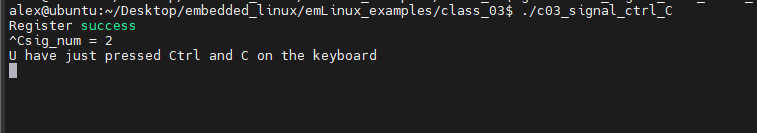
\includegraphics[scale=0.5]{emLinux_c03_signal_ctrl_C}
  \caption{The result of the example}  
\end{figure}



1h20m: phan quyen de chay process, moi cau lenh deu phai xem cai quyen cua minh o dau, day co the gay loi cho chuong trinh cua ban
\\1h27m: phai check sau moi cau lenh, de xem init co thanh cong hay ko, vd char *a = malloc, thi phai check if(NULL != a), neu ko co loi thi moi chay func cua minh
\\ngoai ra thi phai check errno (error number).
\\IMPORTANT: errno only stores the value of the latest process.
\\1h41m: co nhieu process qua thi dung kill -9 process\_id.
\\chu y vao trang thai cua process, T, R+, T means terminated 
\begin{figure}[h]
  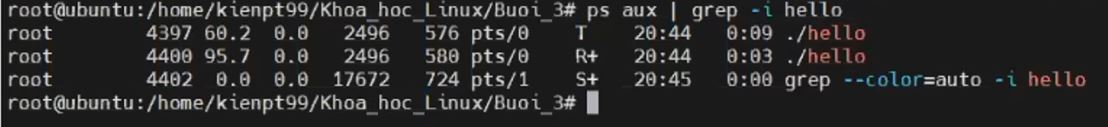
\includegraphics[scale=0.5]{emLinux_c03_multiple_processes}
  \caption{Multiple processes but different status - stop T, running R}  
\end{figure}

google keyword /proc/stat linux from man7.org for more information about the process
\begin{figure}[h]
  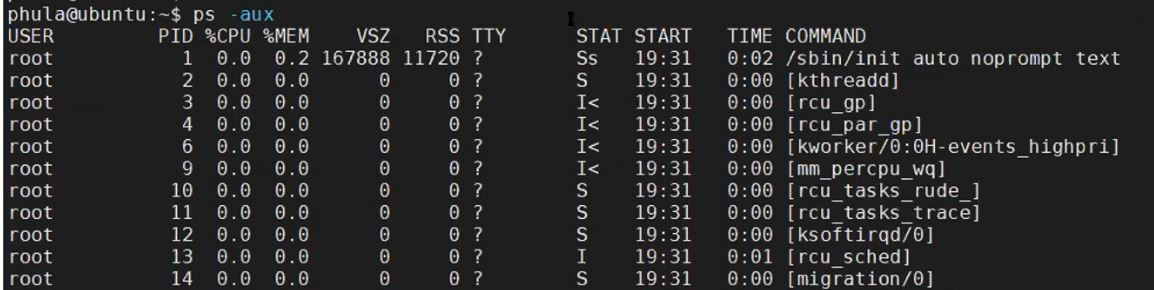
\includegraphics[scale=0.5]{emLinux_c03_fields-of_ps-aux_command}
  \caption{Fields of ps-aux command}  
\end{figure}
\\safe functions to run in the signal handler: slide 11 of 16 of signal ppt.
\\or the keywords: reentrant functions in linux
\\tat ca driver deu co process\_id = 0
\\search keyword 'passing arguments to signal handler' de tim hieu ve pass du lieu vao trong signal handler

\subsection{Vid 4 - Interrupt (Nov 15, 2021)}
tao 1 thread de doc du lieu ngay nay qua thang no.
\\khi nao thi deadlock xay ra
\\gg thread\_create in man7.org
\\sau khi dung lenh pthread\_create thi phai dung lenh pthread\_join
\\1h09m: khi chay nhieu thread, co the bi loi race\_condition
\\1h29m: lenh atomic trong c++, atomic\_increase(a);
\\1h39m: mutex in operating system: khoa 1 chia, mutex\_lock
\\semaphore la khoa nhieu chia
\\1h55m: wrapper function
\\task in RTOS is as same as process in Linux
\\truyen tin giua cac task thi giong voi co che chuyen tin cua process
\\dung lenh time ./mutex thi se in ra tgian chay doan code do.
\\build ra file lib de lam gi.
\\2h26m: end of video




\subsection{Vid 9 - Interrupt (Nov 13, 2021)}

How to connect ssh using the internet
\begin{itemize} 
  \item cam day mang vao cong internet cua beaglebone
  \item sudo apt-get install openssh-server
  \item Ben board beaglebone thi dung lenh sudo ifconfig de xem dia chi ip cua day internet eth0
  \item Tai may windows thi dung mobaXterm, va go lenh ssh debian@192.168.0.43.
  \item sudo \path{nano/etc/ssh/sshd_config}
\end{itemize}


\subsection{Vid 13 - Watchdog (Dec 04, 2021)}
Quy tac 5 buoc de viet driver
\begin{itemize}
  \item Tim hieu hardware 
  \item Tim hieu standard giao tiep giua OS va device file cua module do
  \item Tim hieu template driver
  \item Viet driver
\end{itemize}
scp my\_watchdog.ko debian@192.168.0.43: lenh de copy 1 file tu may ubuntu sang may BBB
\\dung lenh 'sudo su' de login o dang root, sau do
\\insmod my\_watchdo.ko sau moi lan reset
\\dung lenh \path{./main_test} de test watchdog
\\Dat log la dat nhu the nao

\subsection{Vid 14 - Uboot (Dec 11, 2021)}
Tai lieu tra cuu uboot - Uboot reference manual,
link \path{https://hub.digi.com/dp/path=/support/asset/u-boot-reference-manual/}\\
\\File uEnv.txt la cho de config cho uboot
\\Homework: sua lai tgian boot cua uboot, de tgian doi ng dung tu 1s tro thanh 30s. 
Co nhieu cach de sua, build lai uboot va ghi vao the.\\
\\Tra trong reference manual, uboot, page 15, bootdelay
\\Node trong Embedded linux la sao?
\\Buildroot vs Yocto, framework de build la gi. 
Buildroot ra doi truoc nhung Yocto ra doi sau nhung tot hon, tuy theo tinh nang
\\OTA update linux - Mender, co the update app va framework OTA
\\Homework 2: type 'hello Phu', show 'xin chao Phu'

\section{Control Bootcamp - Steve Bruton}

\subsection{Vid 01 - Overview}

We could classify the control into these groups:
\begin{itemize}
  \item Passive Control
  \item Active Control
    \begin{itemize}
      \item Open-loop Control
      \item Closed-loop Control
    \end{itemize}
\end{itemize} 
Why feedbacks?
\begin{itemize}
  \item Uncertainty
  \item Intability
  \item Disturbances Rejection
  \item Efficient Control
    \begin{itemize}
      \item You have to continuously move the inverted pendulum up and down to keep it stable (openloop)
      \item But if you have a good fdback controller, you barely have to control the cart, and the stick is still stable
      \item You only need to control whenever you need it, not all the time
    \end{itemize}
\end{itemize}

\subsection{Vid 02 - Linear System} 
\subsubsection{Linear System $ \dot{X} = A.X, ~with X \in\mathbb{R}^{n} $}


The solution for the equation is 
\begin{equation}
  X(t) = e^{At}.X(0)
\end{equation}
with $X$ is a vector, $A$ is a matrix.
\\Use Taylor series to expand $e^{At}$ 
\begin{equation}
  e^{At} = I + At + \frac{ A^{2}t^{2} }{2!} + \frac{ A^{3}t^{3} }{3!} + \ldots + \frac{ A^{n}t^{n} }{n!}
\end{equation}

But if we have $ A $ is a $5 \times 5$ matrix, calculating $ e^{At} $ is not practical to compute, so we will use eignenvalue and eigenvector of A
\\to get a coordinate transformation from $ X $ coordinates to eigenvector's coordinates.
\\so that it is easier for us to understand the dynamics themselves $ \dot{X} = A.X $ and easier to write down $ e^{At} $

With 
\begin{equation} 
  \dot{X} = A.X
\end{equation}

Use MATLAB to find T, D matrices
\begin{equation}
  [T, D] = eig(A)
\end{equation}

Matrix D is a diaganol matrix
\begin{equation} 
D = \begin{bmatrix}
      $$\lambda_{1}$$ &  &  &\\ 
      & $$\lambda_{2}$$   &  &\\ 
      & & \ddots & \\ 
      & & & $$\lambda_{n}$$
    \end{bmatrix}
  \end{equation}

From D we calculate the $e^{Dt}$  
  \\\begin{equation} 
    e^{Dt} = 
      \begin{bmatrix} 
        $$e^{\lambda_{1}t}$$  &  &  & \\ 
        & $$e^{\lambda_{2}t}$$   &  & \\ 
        & & \ddots & \\ 
        & & & $$e^{\lambda_{n}t}$$
      \end{bmatrix} 
    \end{equation}
\subsubsection{Eignevalue and Eigenvector}
with $A = TDT^{-1}$
\begin{equation}
  \begin{aligned}
    e^{At}  & = e^{TDT^{-1}t} \\
            & = I + At + \frac{ A^{2}t^{2} }{2!} + \frac{ A^{3}t^{3} }{3!} + \ldots + \frac{ A^{n}t^{n} }{n!} \\
            & = TIT^{-1} + TDT^{-1}t + \frac{ TDT^{-1}.TDT^{-1}t^{2} }{2!} + \ldots + \frac{ (TDT^{-1})^{n}t^{n} }{n!}\\
            & = T.[I + Dt + \frac{D^{2}t^2}{2!}] + \frac{D^{3}t^3}{3!} + \ldots + \frac{D^{n}t^{n}}{n!} ].T^{-1}\\
            & = T.e^{Dt}.T^{-1}
  \end{aligned}
\end{equation}  
Try to write the system in this form AT = TD (8:19 timestamp)
\begin{equation}
  \begin{aligned}
    A.T  & = T.D \\
    T^{-1}.A.T  & = T^{-1}.T.D \\
    T^{-1}.A.T & = D
  \end{aligned}  
\end{equation} 

We have
\begin{equation}
  \begin{aligned}
    X &= TZ \\
    \dot{X} &= T\dot{Z} = AX \\
    T\dot{Z} &= AX \\
    T\dot{Z} &= ATZ \\
    T^{-1}T\dot{Z} &= T^{-1}ATZ \\
    \dot{Z} &= T^{-1}ATZ \\
  \end{aligned}  
\end{equation} 

with $ T^{-1}.A.T = D $
\begin{equation}
  \dot{Z} = DZ
\end{equation}
Why do we really need $D$ to be diaganol?
\\Because D now is a diaganol matrix 
so that all the component of $Z$ is fully decoupled to each other.
In another words,
$Z_{1}$ only effects $\dot{Z_{1}}$, $Z_{2}$ only effects $\dot{Z_{2}}$

\begin{equation} 
  D = 
  \begin{bmatrix}
        $$\lambda_{1}$$ &  &  &\\ 
        & $$\lambda_{2}$$   &  &\\ 
        & & \ddots & \\ 
        & & & $$\lambda_{n}$$
  \end{bmatrix}
\end{equation}

\begin{equation}     
  \begin{bmatrix}
    $$\dot{Z_1}$$\\ 
    $$\dot{Z_2}$$\\ 
    \vdots\\
    $$\dot{Z_n}$$ 
  \end{bmatrix}
  =
  \begin{bmatrix}
    $$\lambda_{1}$$ &  &  &\\ 
    & $$\lambda_{2}$$   &  &\\ 
    & & \ddots & \\ 
    & & & $$\lambda_{n}$$
  \end{bmatrix}
  \begin{bmatrix}
    $$Z_1$$\\ 
    $$Z_2$$\\ 
    \vdots\\
    $$Z_n$$ 
  \end{bmatrix}
\end{equation}

The solution for $\dot{Z} = DZ$  is $Z(t) = e^{Dt}.Z(0)$ (13:46 tstamp)
We think immediately in our mind 
when we see the $\dot{X} = AX$
is think about it in eigenvector $X = TZ$
because it is simple for the solution $Z(t)$




\subsubsection{Eigenvector Relationship}
Start with this Taylor series to expand $e^{At}$
\begin{equation}
  e^{At} = I + At + \frac{ A^{2}t^{2} }{2!} + \frac{ A^{3}t^{3} }{3!} + \ldots + \frac{ A^{n}t^{n} }{n!}
\end{equation}
\\The transformation from $e^{At}$ = $Te^{Dt}T^{-1}$ (20:43 tstamp), 
we do this because it is very easy to compute the $e^{Dt}$ due to the diaganol characteristic of matrix D


IMPORTANT: The main idea (concept) is $X(t) = Te^{Dt}T^{-1}.X(0)$, with $X = TZ$
\begin{itemize}
  \item $Z(0) = T^{-1}.X(0)$: mapping the IC from x coordinates to eigenvector coordinates 
  \item Then multiply with $e^{Dt}$ to form $Z(t) = e^{Dt}.T^{-1}.X(0)$: it is intuitive because the dynamics is decoupled already
  \item Then multiply with $T$ to map it back to $X$ coordinates, $X(t) = Te^{Dt}T^{-1}.X(0)$  which is required in the physical world - what we care is x, not z.
\end{itemize}


\subsubsection{Next step}
\begin{itemize}
  \item Analyze the stability using eigenvectors of matrix A
  \item Build discrete model instead of using continuous model $ \dot{X} = A.X $ by discretize the system with $\lambda T$
  \item Add the control Bu part to start controlling the dynamics $\dot{X} = A.X  + B.u$
\end{itemize}


\subsection{Vid 03 - Stability and Eigenvalues}
\begin{equation} 
  \dot{X} = A.X
\end{equation}

Use MATLAB to find T, D matrices
\begin{equation}
  [T, D] = eig(A)
\end{equation}

Matrix D is a diaganol matrix
\begin{equation} 
  D = 
  \begin{bmatrix}
      $$\lambda_{1}$$ &  &  &\\ 
      & $$\lambda_{2}$$   &  &\\ 
      & & \ddots & \\ 
      & & & $$\lambda_{n}$$
  \end{bmatrix}
\end{equation}

\begin{equation} 
  e^{Dt} = 
    \begin{bmatrix} 
        $$e^{\lambda_{1}t}$$  &  &  & \\ 
        & $$e^{\lambda_{2}t}$$   &  & \\ 
        & & \ddots & \\ 
        & & & $$e^{\lambda_{n}t}$$
      \end{bmatrix} 
\end{equation}

\subsubsection{Stability of $\dot{X} = A.X $ }
With 
\\$X(t) = Te^{Dt}T^{-1}.X(0)$
\\$\lambda = a \pm bi$
\\$e^{\lambda t} = e^{at}[cos(bt) \pm isin(bt)]$
\begin{itemize}
  \item if ALL of the REAL parts of all the eigenvalues has $a < 0$ then the system is STABLE
  \item if any of the REAL parts of all the eigenvalues has $a > 0$ then the system is unstable
  \item If any real parts of these lambdas are positive then the $e^{Dt}$ blows up and the $X(t) = Te^{Dt}T^{-1}.X(0)$ will blow up too.
\end{itemize}

\subsubsection{Discrete time model, tstamp 09:14}
$X_{k + 1} = \tilde{A}.X_{k}$
\\$\tilde{A} = e^{A\Delta t}$

We have $X_{0}, \Delta t$, and matrix $A$
\begin{equation}
  \begin{aligned}
    X_{1}  & = {\tilde{A}}^{1}X_{0}, \lambda = 1\\
    X_{2}  & = {\tilde{A}}^{2}X_{0}, \lambda = 2\\
    X_{3}  & = {\tilde{A}}^{3}X_{0}, \lambda = 3\\
    \ldots\\
    X_{N}  & = {\tilde{A}}^{N}X_{0}, \lambda = N
  \end{aligned}  
\end{equation} 

Using polar coordinate to describe the 
\begin{equation}
  \begin{aligned}
    \lambda &= R.e^{i\theta} \\
    \lambda^{N} &= R^{N}e^{iN\theta}
  \end{aligned}
\end{equation}
We see that $\lambda^N$ has the same direction with $\lambda$,
the radius R is powered by N (getting bigger or smaller), and the angle $\theta$ is rotating around
\\So if the radius $R$ of ALL the $\lambda = R.e^{i\theta}$

\begin{itemize}
  \item $ R < 1 $ the system is STABLE because $R^N \rightarrow 0$ when $t \rightarrow \infty$
  \item $ R > 1 $ the system is unstable because $R^N \rightarrow \infty$ when $t \rightarrow \infty$
\end{itemize}
So if all the lambda (also described as vectors) inside the unit circle, then the system is stable
\begin{figure}[h]
  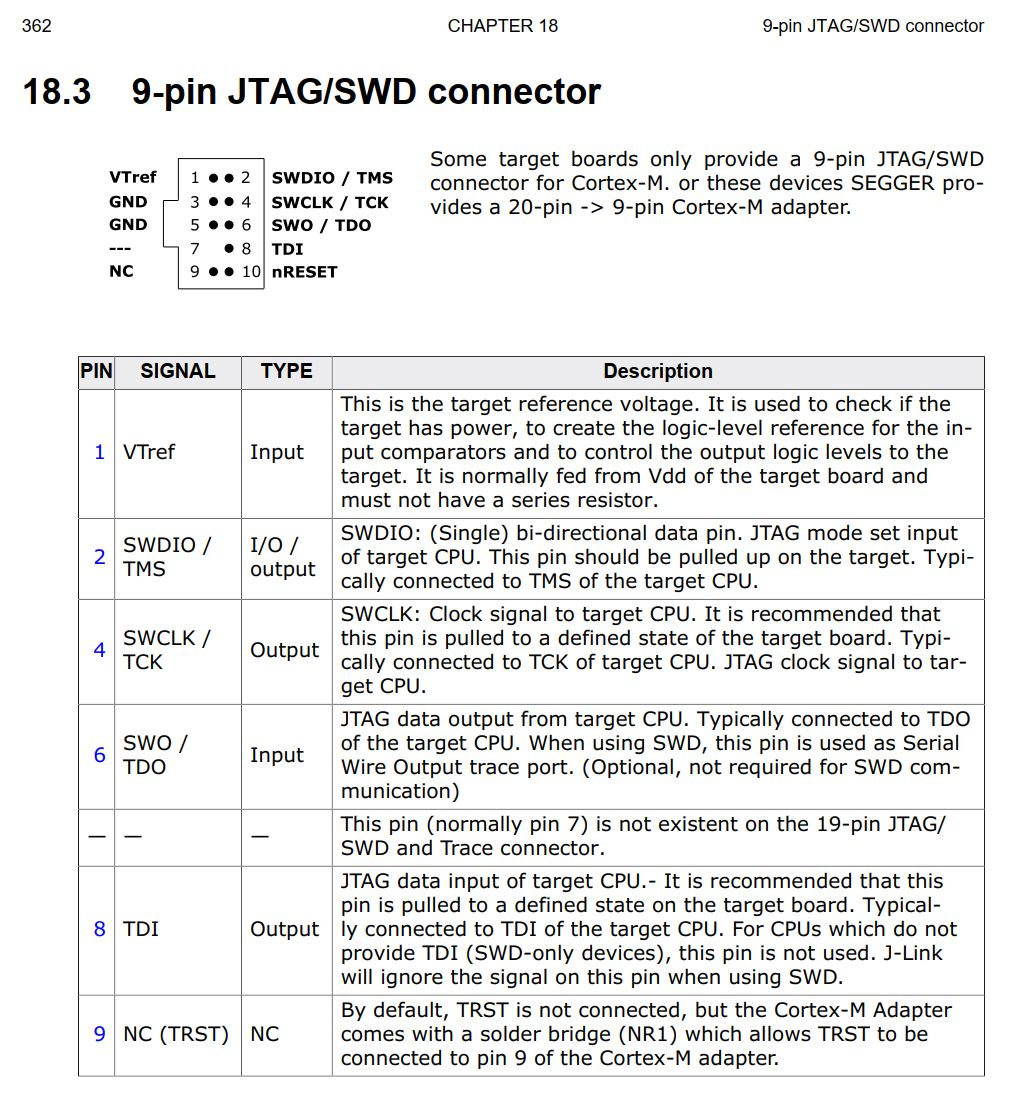
\includegraphics[scale=0.3]{jlink_segger_edu_9pin_JWD-SWD_connector}
  \caption{Pinout of the Jlink segger edu mini}  
\end{figure}

From matrix $\tilde{A}$ - discrete time, we calculate
\\$[ \tilde{T} , \tilde{D}] = eig(\tilde{A})$

Always start with 
\\$ \tilde{A}\tilde{T} = \tilde{T}\tilde{D} $
\\$ \tilde{A}\tilde{T}{\tilde{T}}^{-1} = \tilde{T}\tilde{D}{\tilde{T}}^{-1} $
\\$ \tilde{A} = \tilde{T}\tilde{D}{\tilde{T}}^{-1} $

Plug $ \tilde{A} = \tilde{T}\tilde{D}{\tilde{T}}^{-1}$ into these equations:
\begin{equation}
  \begin{aligned}
    X_{1}  & = {\tilde{A}}^{1}X_{0}, \lambda = 1, {\tilde{D}}^{1}\\
    X_{2}  & = {\tilde{A}}^{2}X_{0}, \lambda = 2, {\tilde{D}}^{2}\\
    X_{3}  & = {\tilde{A}}^{3}X_{0}, \lambda = 3, {\tilde{D}}^{3}\\
    \ldots\\
    X_{N}  & = {\tilde{A}}^{N}X_{0}, \lambda = N, {\tilde{D}}^{N}
  \end{aligned}  
\end{equation} 
We see that the only thing could blow up the system is if the REAL part of ANY lambda in the matrix D is > 0
\begin{equation} 
  \tilde{D} = 
  \begin{bmatrix}
      $$\tilde{\lambda}_{1}$$ &  &  &\\ 
      & $$\tilde{\lambda}_{2}$$   &  &\\ 
      & & \ddots & \\ 
      & & & $$\tilde{\lambda}_{N}$$
  \end{bmatrix}
\end{equation}
The stability of the system is fully depend on the eigenvalues of the matrix A
\begin{itemize}
  \item continuos time, real part must be negative, in the left half plane
  \item discrete time, the eigenvalues must be in the unit circle
\end{itemize}


\subsection{Vid 04 - Linearizing System around fixed point\\ $\dot{X} = f(x) \rightarrow \dot{X} = AX, ~with~ X\in\mathbb{R}^{n}$}
\begin{itemize}
  \item Find the fixed point $\bar{x}$ st $\dot{x} = f(\bar{x}) = 0$
    \begin{itemize}
      \item inverted pendulum, $\bar{x}$ is the top point, 
            without disturbances, the pendulum will stay there forever
      \item pendulum, $\bar{x}$ is the bottom point.
      \item between the Earth and the Sun, $\bar{x}$ 
            the point where the gravitational force of the Sun and the Earth are the same.
    \end{itemize}
   \item Linearize about the fixed point $\bar{x}$ 
    \begin{itemize}
      \item Take partial derivatives
      \item Hartman–Grobman THEOREM, 
            \\https://en.wikipedia.org/wiki/Hartman%E2%80%93Grobman_theorem
            \\We could only linearize the system if the eigenvalues has NON-ZERO REAL PARTS,
            \\IF NOT, the linearization cannot show the dynamics of the system.     
        \begin{equation}
          \frac{Df}{Dx}|_{\bar{x}} = \frac{\partial f_{i}}{\partial x_{j}}
        \end{equation}
      \item examples
        \begin{equation}
          \begin{aligned}
            \dot{X_{1}} &= f_{1}(x_{1}, x_{2}) = x_{1}x_{2} \\
            \dot{X_{2}} &= f_{2}(x_{1}, x_{2}) = {x_{1}}^2 + {x_{2}}^2 \\
            \frac{Df}{Dx} & =
            \begin{bmatrix}
              \frac{\partial f_{1}}{\partial x_{1}}  & \frac{\partial f_{1}}{\partial x_{2}} \\ 
              \frac{\partial f_{2}}{\partial x_{1}}  & \frac{\partial f_{2}}{\partial x_{2}} 
            \end{bmatrix}
            =
            \begin{bmatrix}
               x_{2} &  x_{1} \\ 
              2x_{1} & 2x_{2} 
            \end{bmatrix}
          \end{aligned}
        \end{equation}
    \end{itemize}
\end{itemize}
Examples: The pendulum.
\begin{itemize}
  \item The Equation of Motion
    \begin{equation}
      \ddot{\theta} = -\frac{g}{L}.sin(\theta) - \delta\dot{\theta}
    \end{equation}
  \item Find the fixed point
    \begin{itemize}
      \item Define the state of the system.
        \begin{equation}
          \begin{aligned}
          X &=  \begin{bmatrix} X_{1} \\ X_{2} \end{bmatrix} = 
                \begin{bmatrix}  {\theta} \\ {\dot{\theta} } \end{bmatrix} \\
          \dot{X} &=  \begin{bmatrix} \dot{X_{1}} \\ \dot{X_{2}} \end{bmatrix} = 
                      \begin{bmatrix} \dot{\theta} \\ \ddot{\theta}  \end{bmatrix} =
                      \begin{bmatrix} \dot{\theta} \\ -sin(\theta) -{\delta\dot{\theta}}  \end{bmatrix} = 
                      \begin{bmatrix} X_{2}\\ -sin(X_{1}) -{\delta X_{2} } \end{bmatrix} \\
          \end{aligned}
          \end{equation}
      \item Fixed point $\bar{X}$ so that $\dot{X} = f(\bar{X}) = 0$
        \begin{equation}
            \dot{X} =  
              \begin{bmatrix} 
                X_{2}\\ -sin(X_{1}) -\delta X_{2} 
              \end{bmatrix} 
              =
              \begin{bmatrix} 
                0\\ 0 
              \end{bmatrix}\\
        \end{equation}
        \begin{equation}
            \begin{bmatrix} 
              X_{2}\\ 
              -sin(X_{1})
            \end{bmatrix} 
            =  
            \begin{bmatrix} 
              0\\ 0 
            \end{bmatrix}
        \end{equation} 
        \begin{equation}
          \begin{bmatrix} 
            X_{2}\\ 
            X_{1}
          \end{bmatrix} 
          =  
          \begin{bmatrix} 
            0\\ 0 + k\pi  
          \end{bmatrix}
      \end{equation} 
      In the physical world, there are 2 roots, which are the up position and down position of the pendulum.
      \\There are 2 fixed points:
      \begin{equation}
        \bar{X}_{down} =
        \begin{bmatrix} 
          X_{2}\\ 
          X_{1}
        \end{bmatrix} 
        =  
        \begin{bmatrix} 
          0\\ 0  
        \end{bmatrix}
        and~~ \bar{X}_{up} =
        \begin{bmatrix} 
          X_{2}\\ 
          X_{1}
        \end{bmatrix} 
        =  
        \begin{bmatrix} 
          0\\ \pi  
        \end{bmatrix}
    \end{equation} 
    \end{itemize}
  \item Linearize the system around the fixed points
    \begin{equation}
      \dot{X} =  
      \begin{bmatrix} 
        f_{1}(X_{1}, X_{2})\\ f_{2}(X_{1}, X_{2}) 
      \end{bmatrix}\\
      =
      \begin{bmatrix} 
        X_{2}\\ -sin(X_{1}) -\delta X_{2} 
      \end{bmatrix} 
    \end{equation}
    \begin{equation}
      \frac{Df}{Dx} =
            \begin{bmatrix}
              \frac{\partial f_{1}}{\partial x_{1}}  & \frac{\partial f_{1}}{\partial x_{2}} \\ 
              \frac{\partial f_{2}}{\partial x_{1}}  & \frac{\partial f_{2}}{\partial x_{2}} 
            \end{bmatrix}
            =
            \begin{bmatrix}
               0 &  1 \\ 
              -cos(x_{1}) & -\delta
            \end{bmatrix}  
    \end{equation}  
  \\Subsitute the value of 2 fixed point X into the Jacobian Matrix to find the matrix A for both cases
    \begin{equation}
      \bar{X}_{down} =
      \begin{bmatrix} 
        X_{2}\\ 
        X_{1}
      \end{bmatrix} 
      =  
      \begin{bmatrix} 
        0\\ 0  
      \end{bmatrix}
      ,~~A_{down} =  
      \begin{bmatrix}
        0 &  1 \\ 
       -1 & -\delta
     \end{bmatrix}  
    \end{equation}
    \begin{equation}
      \bar{X}_{up} =
      \begin{bmatrix} 
        X_{2}\\ 
        X_{1}
      \end{bmatrix} 
      =  
      \begin{bmatrix} 
        0\\ \pi  
      \end{bmatrix}
      ,~~A_{up} =  
      \begin{bmatrix}
        0 &  1 \\ 
       1 & -\delta
     \end{bmatrix}  
    \end{equation}
  \item Find the eigenvalues of the 2 matrices A\_up and A\_down, with $\delta = 0.1$
  \\Using Matlab function eig(A)
  \begin{equation}
    A_{down} =  
    \begin{bmatrix}
      0 &  1 \\ 
     -1 & -0.1
   \end{bmatrix}
   , eigenvalues~ = 
    \begin{bmatrix}
      -0.05 + 0.9987i \\ 
      -0.05 - 0.9987i
    \end{bmatrix}  
  \end{equation}
  \begin{equation}
    A_{up} =  
    \begin{bmatrix}
      0 &  1 \\ 
      1 & -0.1
   \end{bmatrix}
   , eigenvalues~ = 
    \begin{bmatrix}
      -1.0512 \\ 
      0.9512
    \end{bmatrix}  
  \end{equation}
  \item Conclusions
    \begin{itemize}
      \item Pendulum in down position is stable, because the real part of 2 eigenvalues are negative
      \item Pendulum in up position is unstable, because there are 1 eigenvalues is positve
      \item The result is as same as we predict before doing this examples
    \end{itemize}
\end{itemize}

\subsection{Vid 5 - Controllability}
Insert the right notations, Xdot, y, u = -kx, xdot = (a-bk)x
\\In real world, people give a matrix A, B, you cannot change it, you could only design the control law to make the system perform better
\\Column Rank and Row Rank
\\Controllability function in Matlab C = ctrb(A,B) only tells you YES or NO, not tell how controllable.
If the rank (C) equals to the number of the states, then the system is controllable.
So we need another way to know how well the system could be controlled
\\Fullstate feedback means you could measure all the elements in the state X
\\IF THE SYSTEM IS CONTROLLABLE, then you could drive the system to any state that you want. and place the pole any where you want.
Link this with the Linear Algebra in Gilbert Strang class of MIT courseware
\\SVD - Single Value Decomposition of a CONTROLLABILITY MATRIX - C, the first part will show you which states of the System
in the order from the easiest to control to the hardest to control.
In other words, which states is easy to reach, which states are not.



\subsubsection{Controllability}
Example of uncontrollable system - tstamp 13:14
How do I modify B to make uncontrollable system to controllable.


\subsection{Vid 6 - Controllability, Reachability, and Eigenvalue Placement }
System is controllable or not?
\\if yes, we could use Pole placement, with any arbitary eigenvalues
\\Reachability, if the column is not depend, assume we 2 vectors in R2, then it is independent,
it could represent the whole plane, whole state of the systems, watch gilbert strang linear algebra.
\\But the limit in reality is the limit in u of physical world. and the linear system disadvantage is
it cannot represent the non-linear factor in the real life.
\\And in linear system equation, we could apply infinity value of U to get the X-dot as big as we want.


\subsection{Vid 7 - Controllability, and the Discrete time Impulse Response }
\subsection{Vid 8 - Degrees of Controllability and Gramians }
\subsection{Vid 9 - Controllability and the Popov-Belevitch-Hautus (PBH) test}

	\subsubsection{remind}
		$\dot{x} = Ax + Bu, ~with~ x\in R^n$ \\
		$C = [B ~ AB ~ A^{2}B ~ \ldots A^{n-1}B]$\\
		$>> rank(ctrb(A,B))$\\

	\subsubsection{The PBH Test}
		The PBH test is (A, B) is controllable if and only iff (iff)
		$rank[(A - \lambda I) ~B] = n$ with every $\lambda$ in the complex plan $\mathbb{C} $ \\
		\\The PBH test
		\begin{equation}
			rank[(A - \lambda I) ~B] = n,~~\forall \lambda \in \mathbb{C}
		\end{equation}
		\\Good question: When will $(A - \lambda I)$ has rank n?
		\\More specificly, when will $(A - \lambda I)$ NOT has rank n(2:43)?
		\\$(A - \lambda I)$ is deefficient, when the determinent of the $(A - \lambda I)$ equals to 0.
		It is the determient equation \begin{equation}  |(A - \lambda I)| = 0 \end{equation}
		\\This equation satisfied with at most $\lambda$ is the eigenvalues of matrix A.
		\\If $\lambda$ is not the eigenvalues of matrix A, then the $(A - \lambda I)$ alone has the rank n,
		and we DO NOT really need the matrix B in the $[(A - \lambda I) ~B]$ to have $rank[(A - \lambda I) ~B]$ = n.\\

	\subsubsection{The PBH Test - Important Conclusions}
		\begin{itemize}

		\item $rank(A - \lambda I) = n $ except for the eigenvalues $\lambda$.
				\\It means we only need to test at eigenvalues, 
				because $(A - \lambda I)$ has rank n if $\lambda$ is not the eigenvalues of matrix A (3:50)
				\\ So we reduce from testing for the whole complex plane $\mathbb{C}$ down to only testing
				at the eigenvalues of matrix A.
		\item B needs to have some components in each eigenvector (of matrix A) direction.
				\\If we pick $\lambda$ as a eigenvalues of matrix A and plug it into the $(A - \lambda I)$,
				we see that the $(A - \lambda I)$ is rank deefficient, and in which direction that
				$(A - \lambda I)$ is rank deefficient?
				\\The answer is, we look at the Nullspace of $(A - \lambda I)$, which is the eigenvector 
				of $(A - \lambda I)$. The $(A - \lambda I)$ is rank deefficient in EXACTLY the direction
				of the eigenvector. And the eigenvector is the reason that makes $(A - \lambda I)$ equals to 0.
				\\We see that in order to have $rank(A - \lambda I) = n $, when $(A - \lambda I) = 0$
				in some eigenvector directions of A, then the matrix B must complement for matrix A, or matrix B
				must at least has some component in all of the eigenvector directions to make $rank[(A - \lambda I) ~B] = n$.
		\item (ADVANCED) if B is a random vector, in another word, if B = randn(n,1), then (A,B) will be
				controllable with high probability.\\
				
				B cannot be aligned with ONLY ONE eigenvector of matrix A because $rank[(A - \lambda I) ~B]$ will be$ = n $
				for that specific $\lambda$, and for the other $\lambda$, the matrix B will not make $rank[(A - \lambda I) ~B] = n$
				So that B must at least has some component in EVERY EIGENVECTOR of matrix A in order to make 
				$rank[(A - \lambda I) ~B] = n$ with all the $\lambda$ in the complex plan $\mathbb{C}$ ($\forall \lambda \in \mathbb{C}$)\\
				
				A random vector B $\in R^n$, with HIGH PROBABILITY, it has a little bit in in ALL of those eigenvector direction of MATRIX A.
				And it is VERY EXTREMELY UNLUCKY for B to be aligned with ONLY one, two or a few eigenvector direction.
				So that it is a high probability that a random B will make , $rank[(A - \lambda I) ~B] = n $
				with all the $\lambda$.\\
				
				Even for the very high dimension of matrix A (milion by milion dimensional system),
				if I pull out a random vector B from $R^n$, then with the HIGH PROBABILITY, it is going to be able
				to controll all the states $x$ of the system $\dot{x} = Ax + Bu, ~with~ x\in R^n$

		\item The PBH test tell me that, with a GIVEN MATRIX A, what is the minimal number of columns B, 
				minimum of control actuators that we need in order to make the system $\dot{x} = Ax + Bu$ CONTROLLABLE.\\
		
				If there are 2 eigenvector direction in the null space of this operator $(A - \lambda I)$, 
				then we need matrix B has 2 columns in order to fill in the null space and have a rank n. 
				That is also mean you need 2 CONTROL INPUTS for your system.

		\item WE USE THIS TEST TO THINK ABOUT HOW CONTROLLABLE IS THE SYSTEM?\\
				In case the system in the gray area, What if you have 2 different eigenvalues that is really close,
				or 2 eigenvectors but it is nearly the same (parallel) but it is not.\\
				The >>rank(ctrb(A,B)) from MATLAB tell us the system is controllable (binary result), but in fact,
				the system is approximately DEGENERATED, and be BARELY CONTROLLABLE.\\
				\\SOLUTION: we want to have MULTIPLE COLUMNS of matrix B to boost the control authority of the system.
		\end{itemize}




random vector la gi, nullspace, subspace


\subsection{Vid 10 - Cayley-Hamilton Theorem}

$\dot{x} = Ax + Bu, ~with~ x\in R^n$ \\

\subsection{Vid 12 - Inverted Pendulum on a Cart}
We have 2 states but due to Newton 2nd law, we have 4 (double) coupled ODEs (2:15)


Because the rank of the Controllability matrix is 4,
I can span all of my state space with this Controllability subspace and that means
I can actually develop a controller to control the system.


Set up the problem, identify matrix A, B, and the initial condition.
Find the fixed points of the system.
Linearize the system at the fixed point.
Analyze the stability of the system with eig(A) and the Controllability with rank(ctrb(A,B))

\subsection{Vid 13 - Pole Placement for the Inverted Pendulum on a Cart}
We cannot move the poles (eigenvalues) of the feedback system to the left half plane forever
because
\begin{itemize}
	\item 	the control power of the actuator u is limit, 
			not unlimit to meet up with the control demand from the controller
	\item 	when the response is fast, the dynamics of the system is out of the range
			when we linearize the non linear system. So that the controller we built
            for the linearized system failed.			
\end{itemize}

\subsection{Vid 13 - Linear Quadratic Regulator (LQR) Control for the Inverted Pendulum on a Cart}

What is the math behind pole placement and the LQR?

\section{MATLAB SIMULINK}

\subsection{Dec 10, 21}

We could make different color for the time legend, 
according to the video in the link: 
\path{https://www.youtube.com/watch?v=8jB0D7CD5Z8}\\

How to make cascaded simulation in simulink?\\

How to use git for simulink, matlab?
\section{STM32}

\subsection{Nov 04, 2021}

CubeIDE vs CubeMX differences?
\\add path trong environments, edit file path, link to the folder store the make (cygwin), git, etc. so we could use it in the terminal of the visual code.


\subsection{Nov 05, 2021}
Equivalences at tstamp 7:15

reference nhung noi de thay doi file makefile tuy theo loai chip trong video 02 - toanchung

\subsection{Nov 29, 2021}

Compare JTAG vs SWD
The other good thing about SWD is you can use the serial wire viewer for your printf statements for debugging.
\begin{figure}[h]
  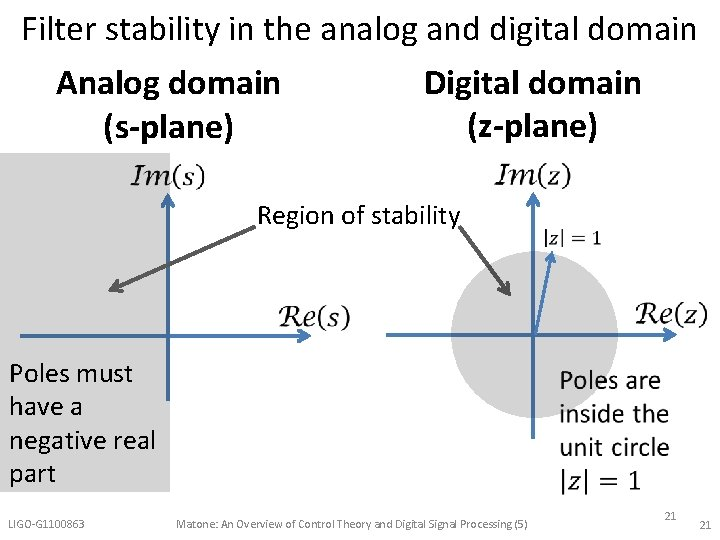
\includegraphics[scale=0.3]{control_bootcamp_stable_region_in_s_and_z_domain}
  \caption{Mapping stable region between s-continuos and z-discrete domain}  
\end{figure}

\section{C - PROGRAMMING}
Pointers\\
array[ ] different ? is it a 2 dimension, 3 dimensions array?\\
int * const array, use array name, so it is 1 dimension (single subscripted array?)\\
what is the principle of least privilege?
opreands la gi?\\
Portability Tip 7.3\\
Most computers today have 2-byte or 4-byte integers. Some of the newer machines use 8-
byte integers. Because the results of pointer arithmetic depend on the size of the objects a
pointer points to, pointer arithmetic is machine dependent.\\
Pointers are valid operands in arithmetic expressions, assignment expressions and comparison expressions.\\
Arithmetic operations: cac phep tinh toan hoc, basics: + - x / 
\\
how to know the system is 2, 4 or 8 byte systems?
\\
Pointers can be compared using equality and relational operators, but such comparisons are meaningless unless the pointers point to elements of the same array
\\
Array element b[3] can alternatively be referenced with the pointer expression: *( bPtr + 3 )\\
The parentheses are necessary because the precedence of * is higher than the precedence of + .
\\
string vs character array?\\
What is the end char of the string? null? "'slash 0'?" how to see it?\\
const int * xPtr \\
int * const xPtr \\
const char * const s2\\
\\DESIGN STEP
\\first think about the flow of the codes
\\which variable is fixed, should not be changed by mistakes, then use the qualifier const
\\should only pass the variable by value and return ONLY ONE value in each function for the principle of least of privilege
\\should not change the value of the variable inside the function if you dont really need to do that

%\begin{figure}[h!]
%    \centering
%    \includegraphics[scale=1.7]{universe}
%    \caption{The Universe}
%    \label{fig:universe}
%\end{figure}
\section{WHAT'S NEXT}

\subsection{Dec 10, 21}
\begin{itemize}
    \item Watch 47 videos control Bootcamp - Bruton
    \item Answer Questions
    \item Fix GG Calendar - Done
    \item Watch ( 8-12 / 47 ) videos control Bootcamp - Bruton
\end{itemize}

\subsection{Dec 06, 21}
\begin{itemize}
    \item Change ticket time - Done
    \item Sign Offer - Done
    \item Confirm the info of Gusto - Done
    \item Watch ( 1-8 / 47 ) videos control Bootcamp - Bruton
\end{itemize}

\subsection{Nov 25, 21}
\begin{itemize}
    \item xem het video cua Embedded Linux, 1 ngay 2 videos, 5,6 
    \item xem video Linear Algebra 2 videos 1 ngay, 8 9 10
    \item Github for simulink va matlab code
    \item setup cho stm32 toan chung
\end{itemize}

% %\chapter*{References}
%\addcontentsline{toc}{chapter}{\protect\numberline{}{References}}
%\paragraph{}

% \bibliographystyle{plain}
\bibliography{ref}
\bibliography{References}
% ``I always thought something was fundamentally wrong with the universe'' \citep{adams1995hitchhiker}

% \addcontentsline{toc}{chapter}{Bibliography}

% \begin{singlespace}
% \bibliographystyle{plain}

% \bibliography{references}
% \end{singlespace}
% \printbibliography[title=References]


\end{document}
